
This is the introduction.

LaTeX is a document markup language and document preparation system for the TeX typesetting program.

It is widely used by mathematicians, scientists, philosophers, engineers, and scholars in academia and the commercial world, and by others as a primary or intermediate format (e.g. translating DocBook and other XML-based formats to PDF) because of the quality of typesetting achievable by TeX. It offers programmable desktop publishing features and extensive facilities for automating most aspects of typesetting and desktop publishing, including numbering and cross-referencing, tables and figures, page layout and bibliographies.

LaTeX is intended to provide a high-level language to access the power of TeX. LaTeX essentially comprises a collection of TeX macros, and a program to process LaTeX documents. Since TeX's formatting commands are very low-level, it is usually much simpler for end-users to use LaTeX.

LaTeX was originally written in 1984 by Leslie Lamport at SRI International and has become the dominant method for using TeX—few people write in plain TeX anymore.

LaTeX is based on the idea that authors should be able to focus on the meaning of what they are writing, without being distracted by the visual presentation of the information. In preparing a LaTeX document, the author specifies the logical structure using familiar concepts such as chapter, section, table, figure, etc., and lets the LaTeX system worry about the presentation of these structures. It therefore encourages the separation of layout from content, while still allowing manual typesetting adjustments where needed. This is similar to the mechanism by which many word processors allow styles to be defined globally for an entire document, or the CSS mechanism used by HTML.

\begin{figure}
\begin{center}
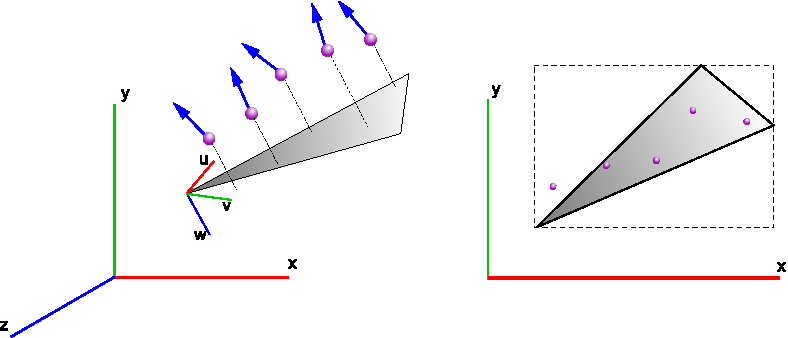
\includegraphics[height=40mm]{example_figure.pdf}
\captionfonts
\caption[This is a figure]{This is an example figure.  This graphic was drawn in InkScape (http://www.inkscape.org/), a free vector drawing application.  Figures can be exported from InkScape as PDF images or as EPS (depending upon if you want LaTeX to generate a PDF or a PostScript document.)}
\label{fig:inkscape-example}
\end{center}
\end{figure}

